\chapter*{Executive Overview}
This report aims to provide the reader with a compelling design for an Inter-Urban Air Mobility (UAM) Vehicle concept, which is supposed to revolutionise short-to-medium distance transportation.
This is achieved through the design and operation of an electric Vertical Take-off and Landing(eVTOL) Vehicle used for travelling within and in between urban areas.
Since a very important issue of Urban Mobility is the last-mile issue, this project focuses on designing a vehicle with a reduced ground footprint.
Additionally, considering the threats that humanity faces in the near future, the environmental footprint should also be minimised. The Mission Need Statement (MNS) and Project Objective Statement (POS) are formulated as follows:

\paragraph{MNS:}“\textit{Achieve Sustainable Inter-Urban Air Mobility with a low ground footprint vehicle.}”
\vspace{-5mm}
\paragraph{POS:}“\textit{Design a low ground footprint, sustainable, urban transwing electric Vertical Take-Off and Landing vehicle within production costs of 2000000 EUR, by 10 students in 10 weeks time.}”

%In order to showcase how the final concept for the eVTOL vehicle is chosen, this report shall consist of several sections. First and foremost, the project logic is made clear with the help of the organisational structure as well as several project logic diagrams. Afterwards, the mission profile is determined to define the operational mission. The concepts are then analysed and preliminarily sized, followed by performing a detailed trade-off which shall lead to the choice of a single concept for detailed design. To prove that the choice of the final design is justifiable, a comprehensive sensitivity analysis as well as Verification and Validation procedures are performed. Additionally, a detailed Technical Risk Assessment is performed to properly assess the risks that this project as well as the chosen design present. Lastly, in order to ensure the success of the design, a production plan is defined, accompanied by a Sustainable Development Strategy as well as an analysis of the interfaces of the design.

% \section*{Organisation}

%In order to ensure that the flow of the project is continuous and smooth, enabling the completion of the project in the specified time frame, it is important to establish a clear organisation of the team members as well as a well-thought-out work distribution. First and foremost, the relevant roles of each of the team members is defined through the use of the Organisational Breakdown Structure. Afterwards, the project Logic Diagrams is showcased to the reader.

% \subsection*{Organisational Breakdown}
% When it comes to the Organisational Breakdown Structure(OBS), the responsibilities and direct communication lines can easily be defined through the use of such of tool.  In the OBS, the significant roles that have to be performed during the project is presented alongside the initials of the relevant team members that is responsible for that role. Based on the OBS the following roles were defined:
% \begin{figure}[H]
%     \centering
%     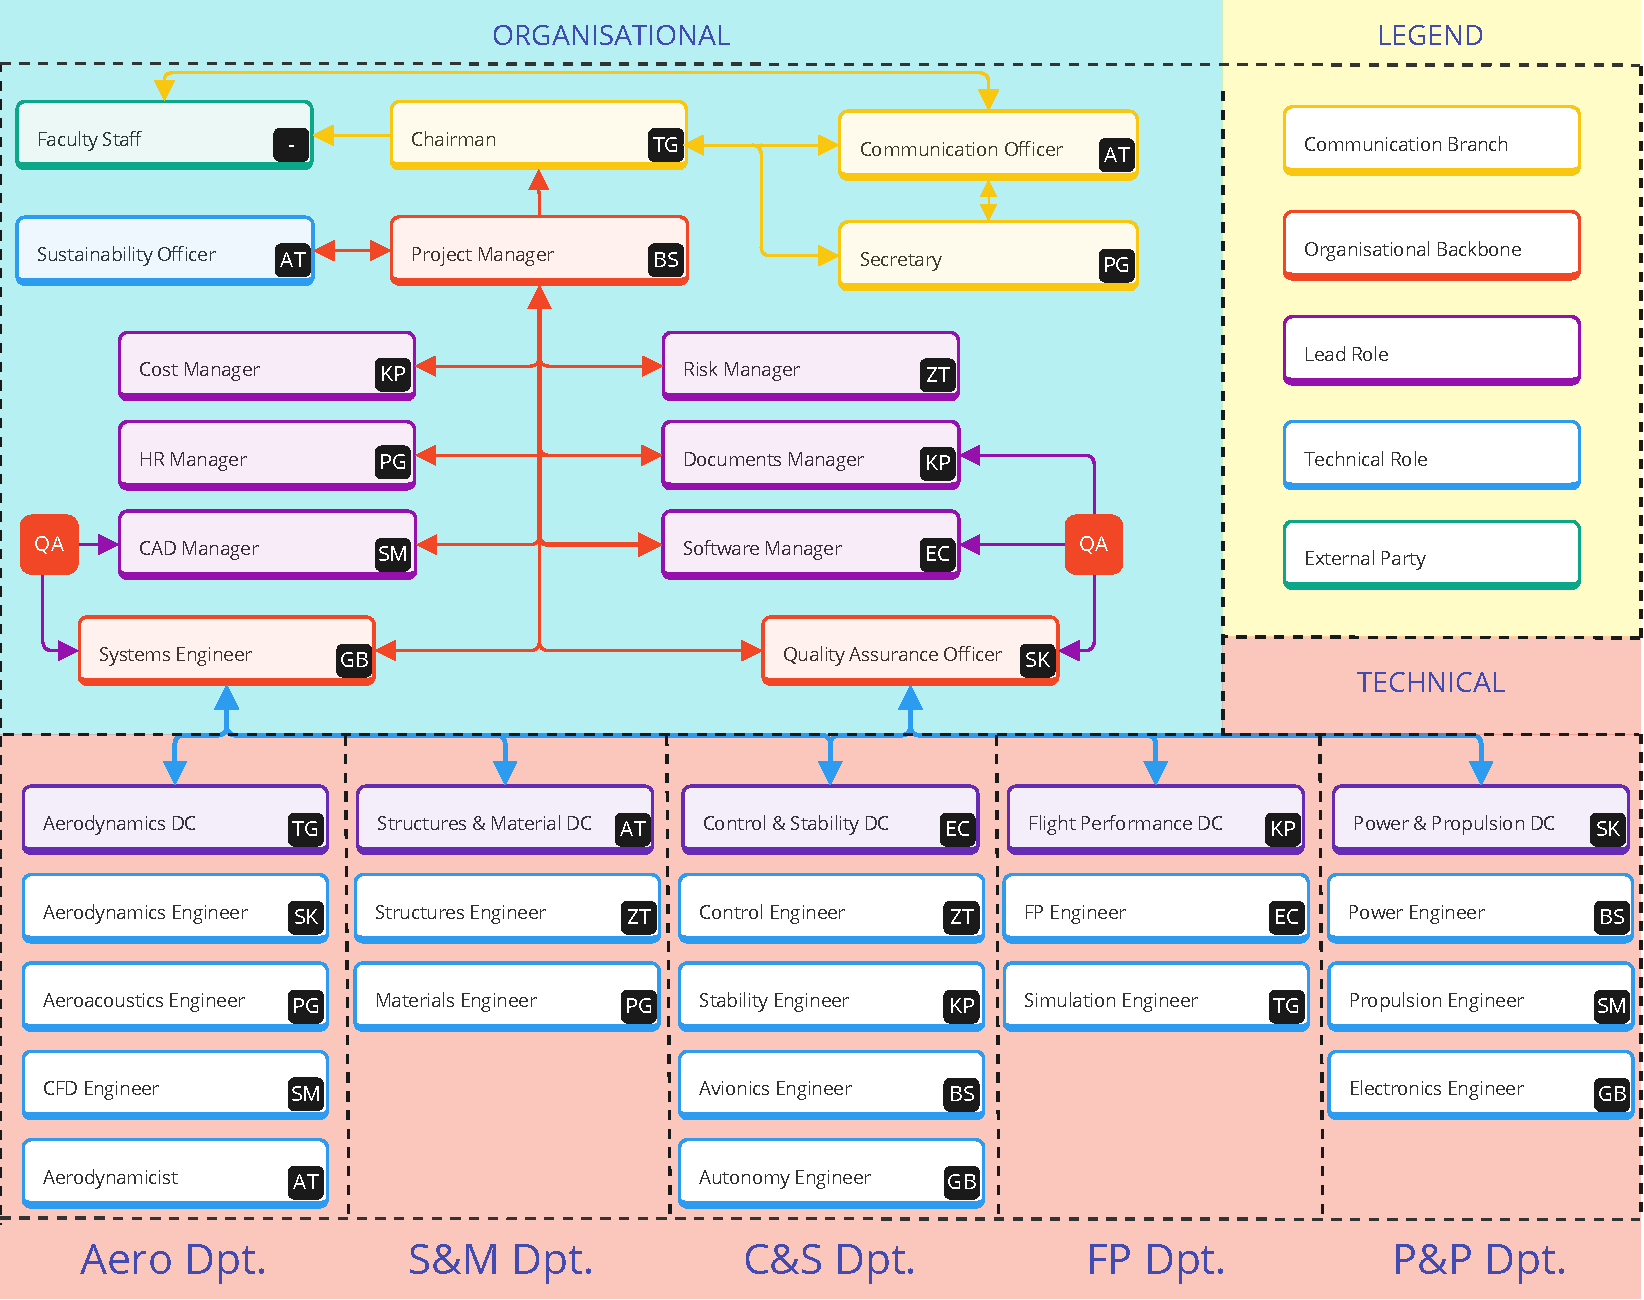
\includegraphics[width=1.0\linewidth]{figures/Organogram.pdf}
%     \caption{Organisational breakdown structure}
%     \label{fig:organogram}
% \end{figure}
\section*{Project Logic Diagrams}
In order to ensure the success of the project, it is important to determine the logic and flow of the different phases of the design.
Several tools are employed for this, such as a Work Flow Diagram, the Work Breakdown Structure, and a Gantt Chart.
This shall ensure a fair distribution of workload among the members of the team and enable monitoring of the progress of each of the tasks. A reduced Work Flow Diagram is presented in \Cref{fig:WFD_red} showcasing the different design phases, the relationship between them, and the expected deliverables.
\begin{figure}[H]
    \centering
    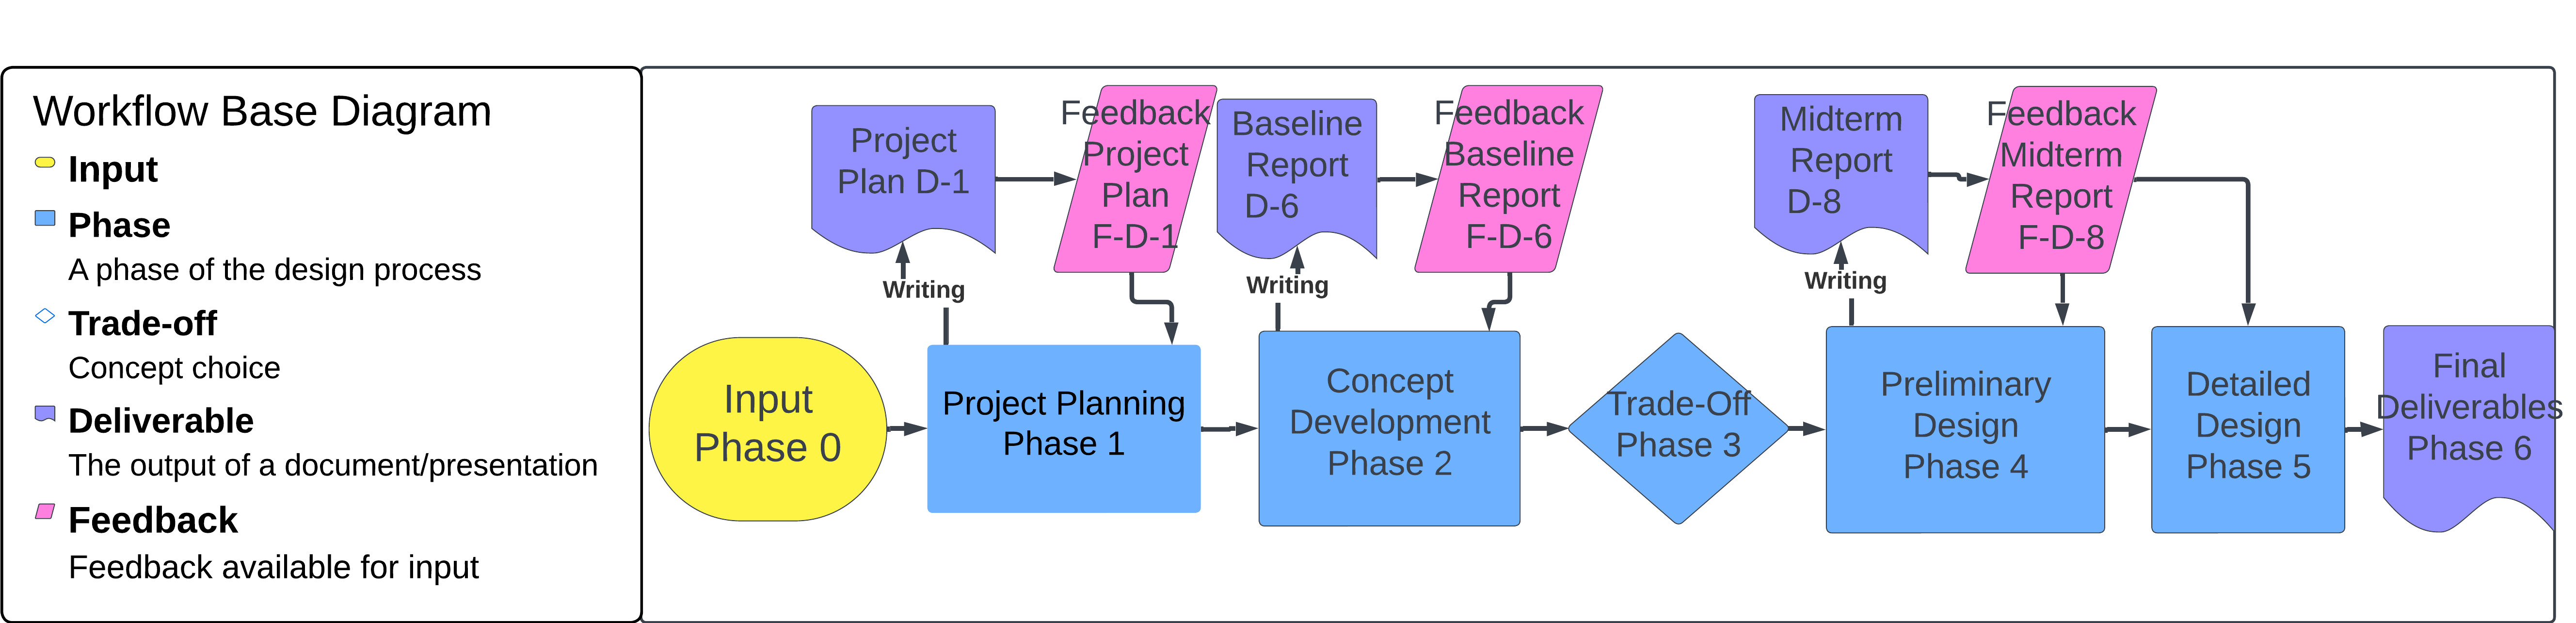
\includegraphics[width=\linewidth]{figures/brad.jpeg}
    \caption{Reduced work flow diagram}
    \label{fig:WFD_red}
\end{figure}

\section*{Mission Profile}
In order to be able to understand the operation of the eVTOLs and to enable proper concept generation, it is important to determine the mission profile of the desired vehicle.
To construct the mission profile, additional literature on eVTOLs and UAM has been consulted (\cite{potential90uam,UAMroland}).
The needs of the potential customers, as well as the competitors in the current UAM market, were also considered.

The mission starts with a vertical take-off phase from a vertiport in an urban area. Here, the aircraft ascends in VTOL (rotorcraft) configuration until the transition altitude is reached to clear all obstacles.
After transitioning to cruise (wing-borne) configuration, the aircraft climbs to approximately 500 meters.
This is followed by the cruise phase, which has the highest duration and is constrained by airspace regulations, vehicle range and air traffic.
The vehicle then starts descending, transitions back to VTOL configuration and lands at the destination.
In case of unexpected schedule disruptions, hovering, loitering or diverting may be required.

\section*{Concepts generation}
% The most important phase of any design project is concept generation. Performing this phase in a proper manner enables the team to come up with a feasible and efficient design, leading to a better-expected output of the project. Thus, it is imperative that each and every concept that can be thought of has to be included in the Design Option Tree and then assessed in order to ensure the feasibility of the design choices that is traded off.
In order to consider multiple design options, it is critical to assess the subsystems that are most influential for the development of the final configuration. Three different design option trees(DOTs) are thus constructed.
Wing configuration, ground footprint reduction methods, and different propulsion systems have been considered. The resulting DOTs can be seen in \Cref{fig_oe:DOTs_subsystems}.

\begin{figure}[H]
    \centering
    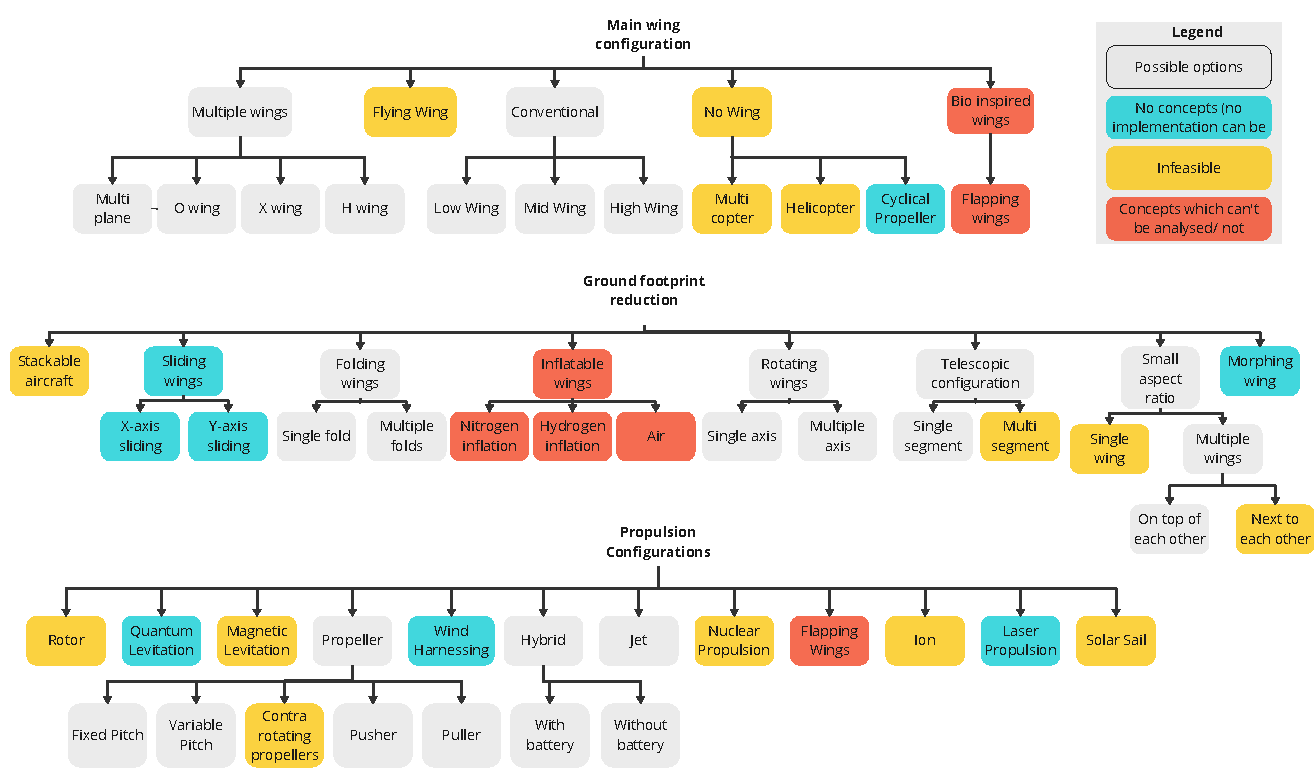
\includegraphics[width=1\linewidth]{figures/AE3200 DOT subsystems.pdf}
    \caption{Design option trees of subsystems}
    \label{fig_oe:DOTs_subsystems}
\end{figure}

A complete configuration design option tree was conceptualised based on the subsystem design option trees.
After analysis and pruning of the options, the four concepts showcased in \Cref{fig_oe:Concept_sketches} were considered to be feasible and potentially well-performing options. These concepts are thus brought forward to be analysed and traded off.

\begin{figure}[h]
    \centering
    
\begin{subfigure}[b]{0.49\textwidth}
    \centering
    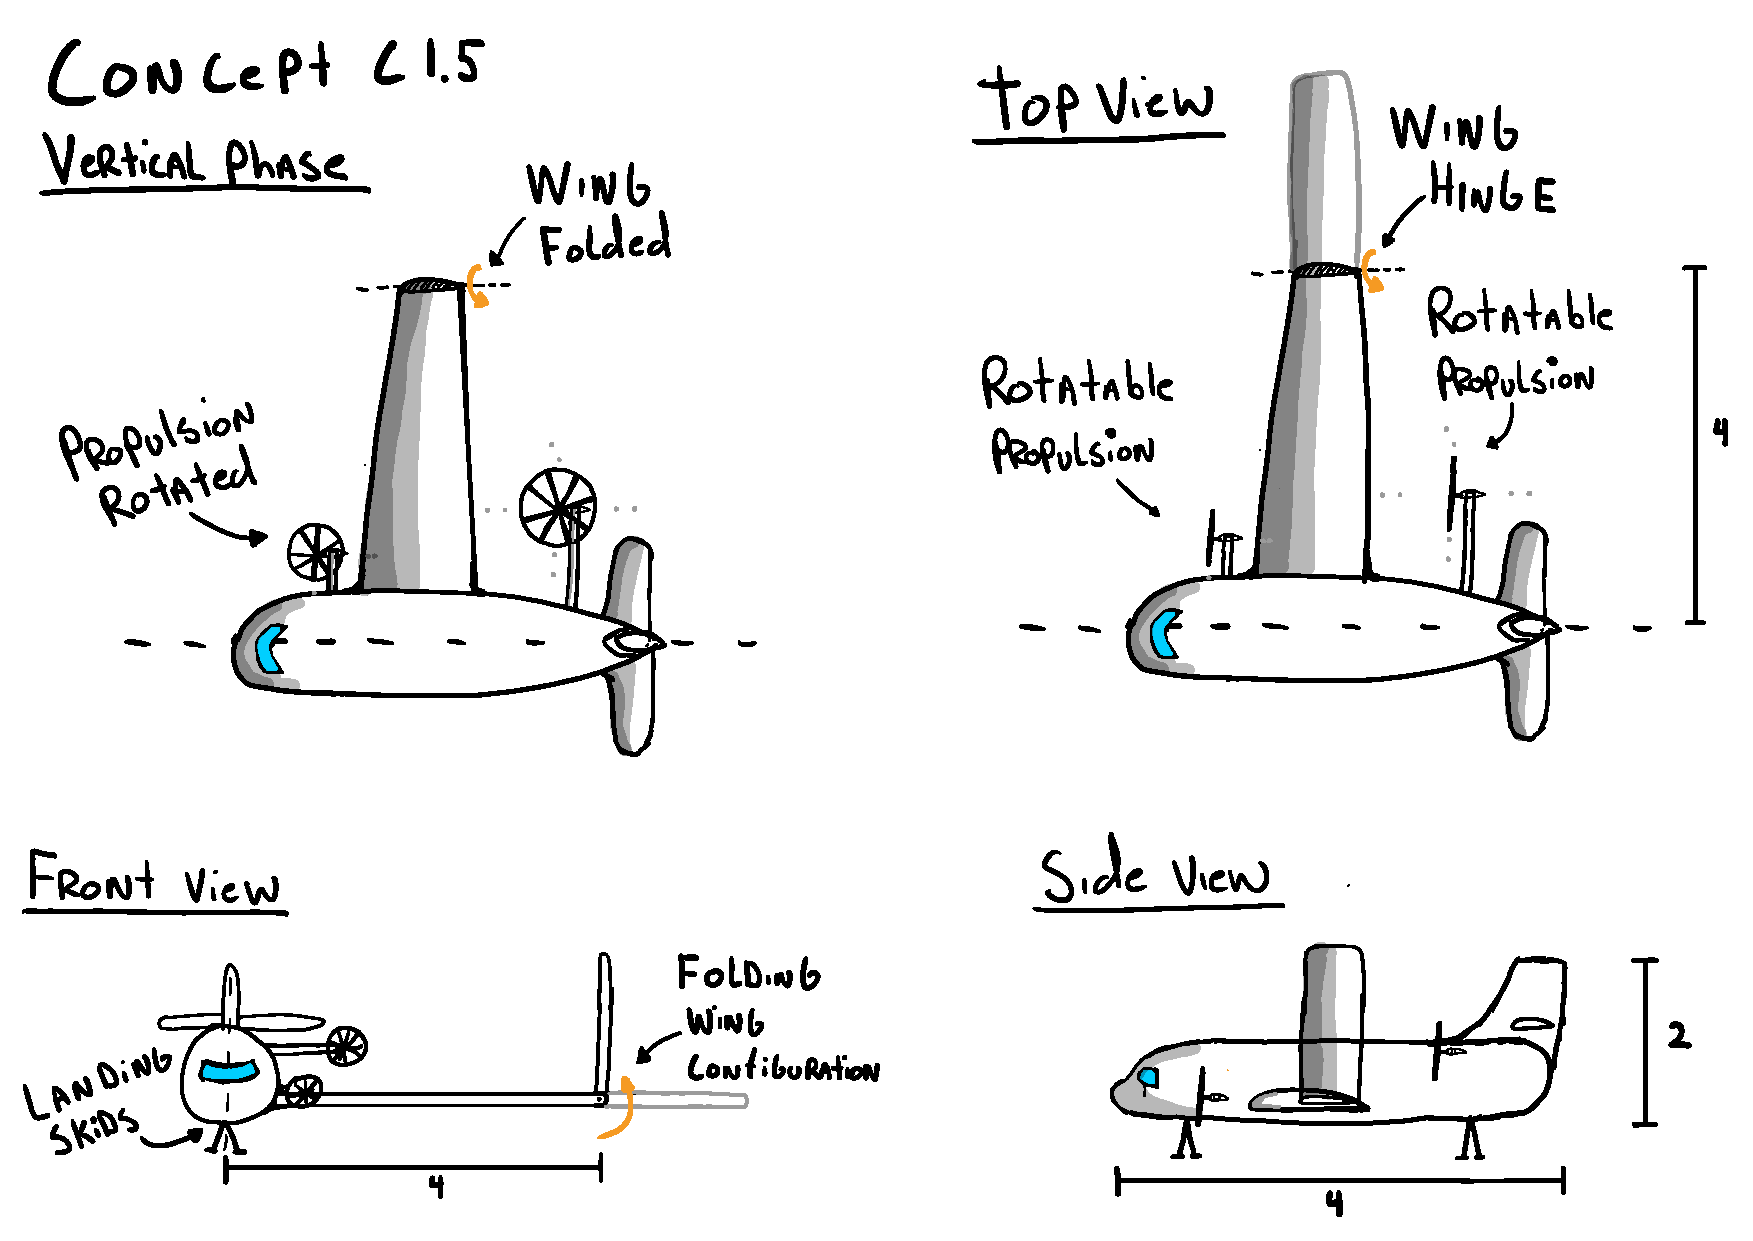
\includegraphics[width=1\linewidth]{figures/Concepts/Concept C1.5 v3.pdf}
    \caption{Concept C1.5: Winged Rotorcraft}
    \label{fig_oe:ConceptC1.5}
\end{subfigure}
~
\begin{subfigure}[b]{0.49\textwidth}
    \centering
    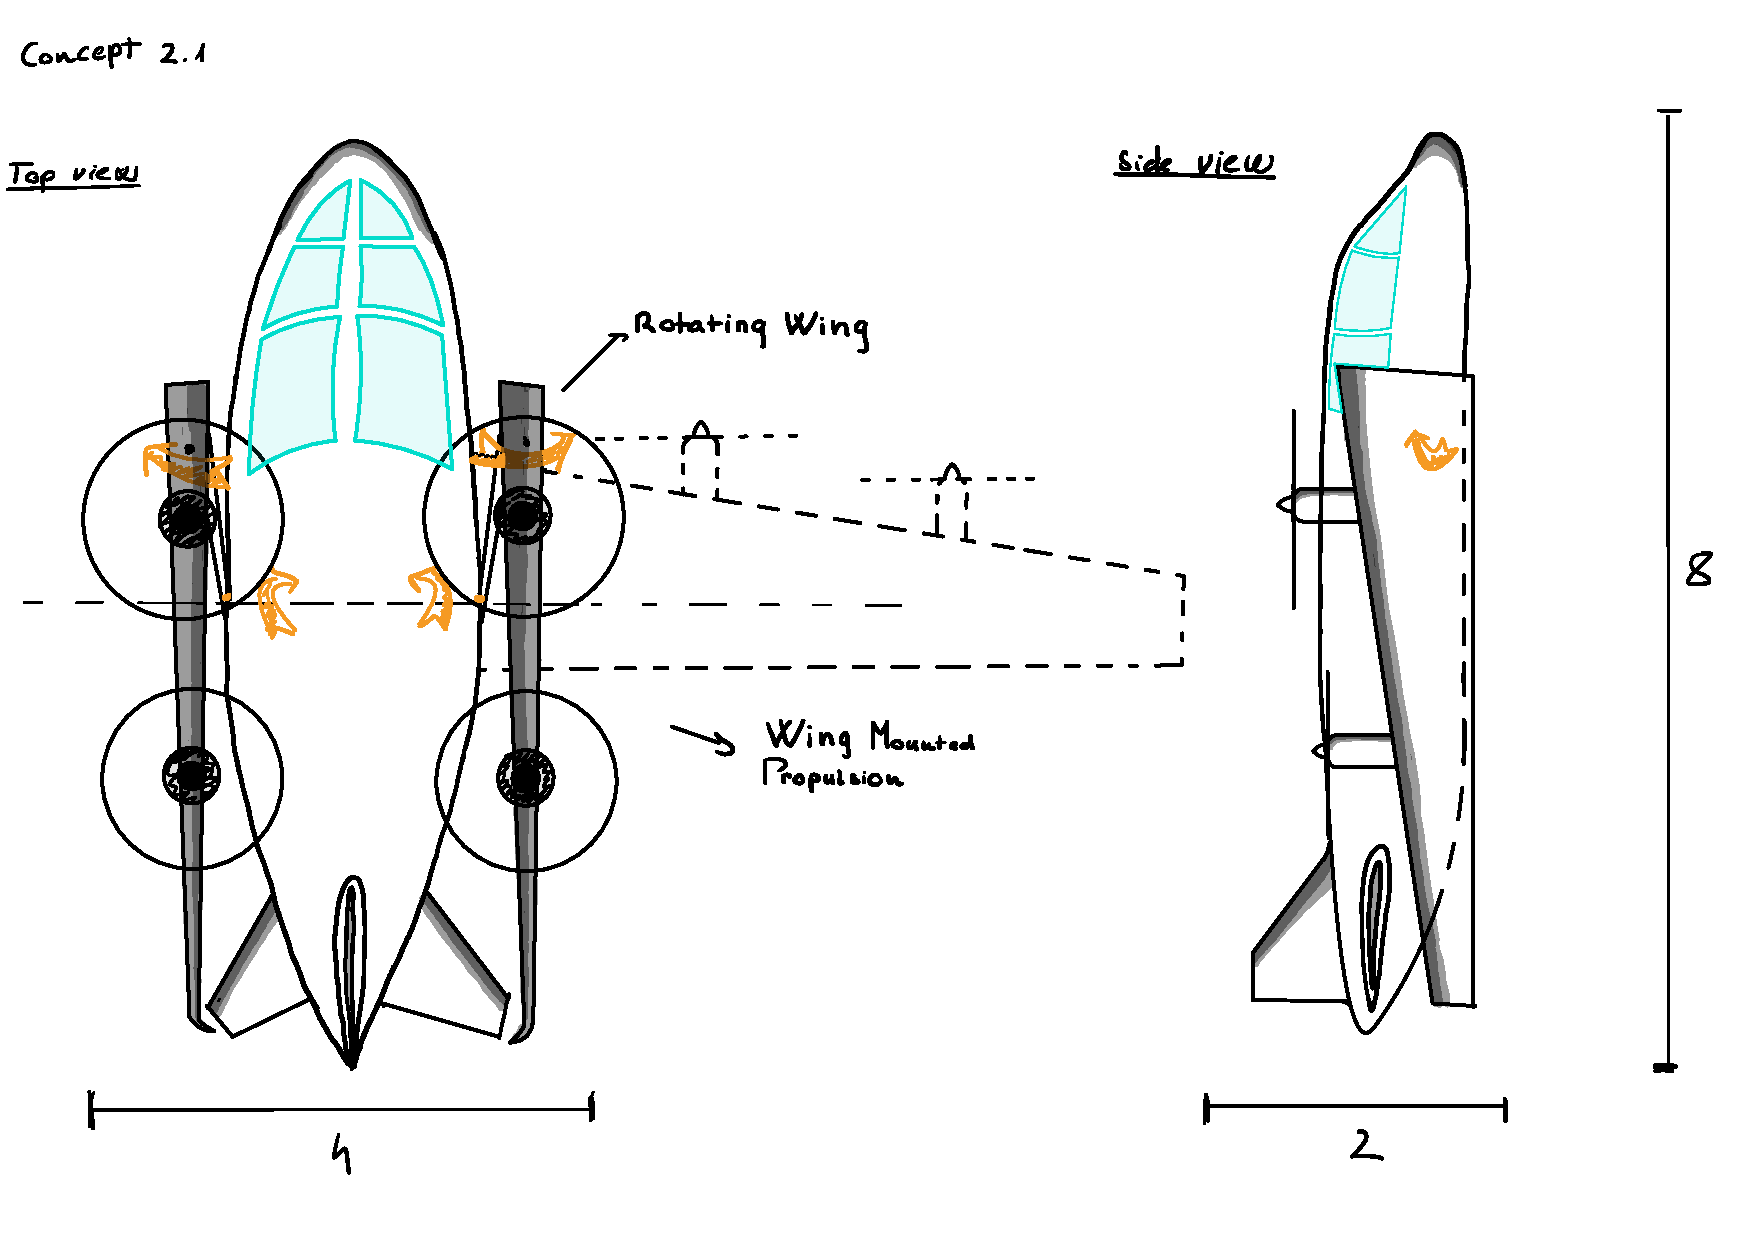
\includegraphics[width=1\linewidth]{figures/Concepts/Concept C2.1 v2.pdf}
    \caption{Concept C2.1: Rotating Wing}
    \label{fig_oe:ConceptC2.1}
\end{subfigure}
~
\begin{subfigure}[b]{0.49\textwidth}
    \centering
    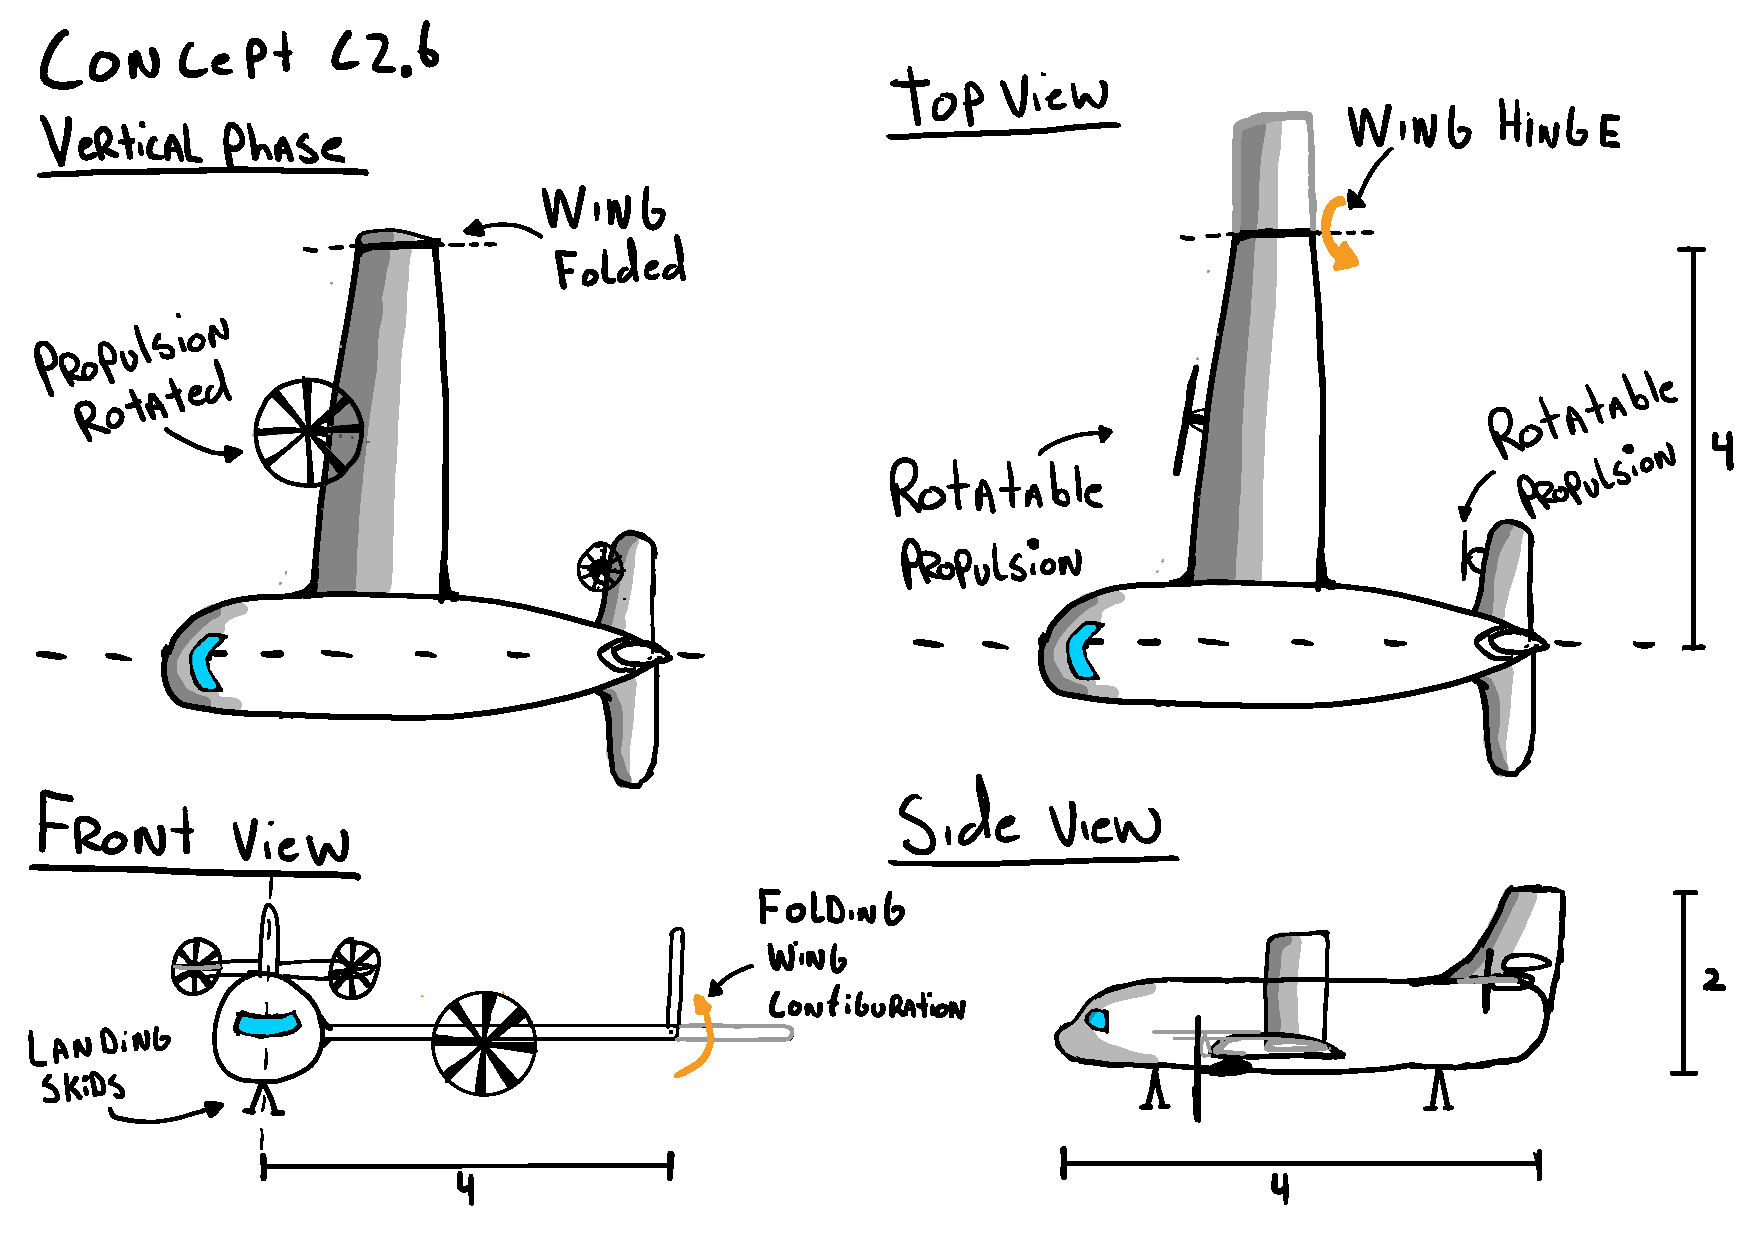
\includegraphics[width=1\linewidth]{figures/Concepts/Concept C2.6 v3.pdf}
    \caption{Concept C2.6: Folding Wing}
    \label{fig_oe:ConceptC2.6}
\end{subfigure}
~
\begin{subfigure}[b]{0.49\textwidth}
    \centering
    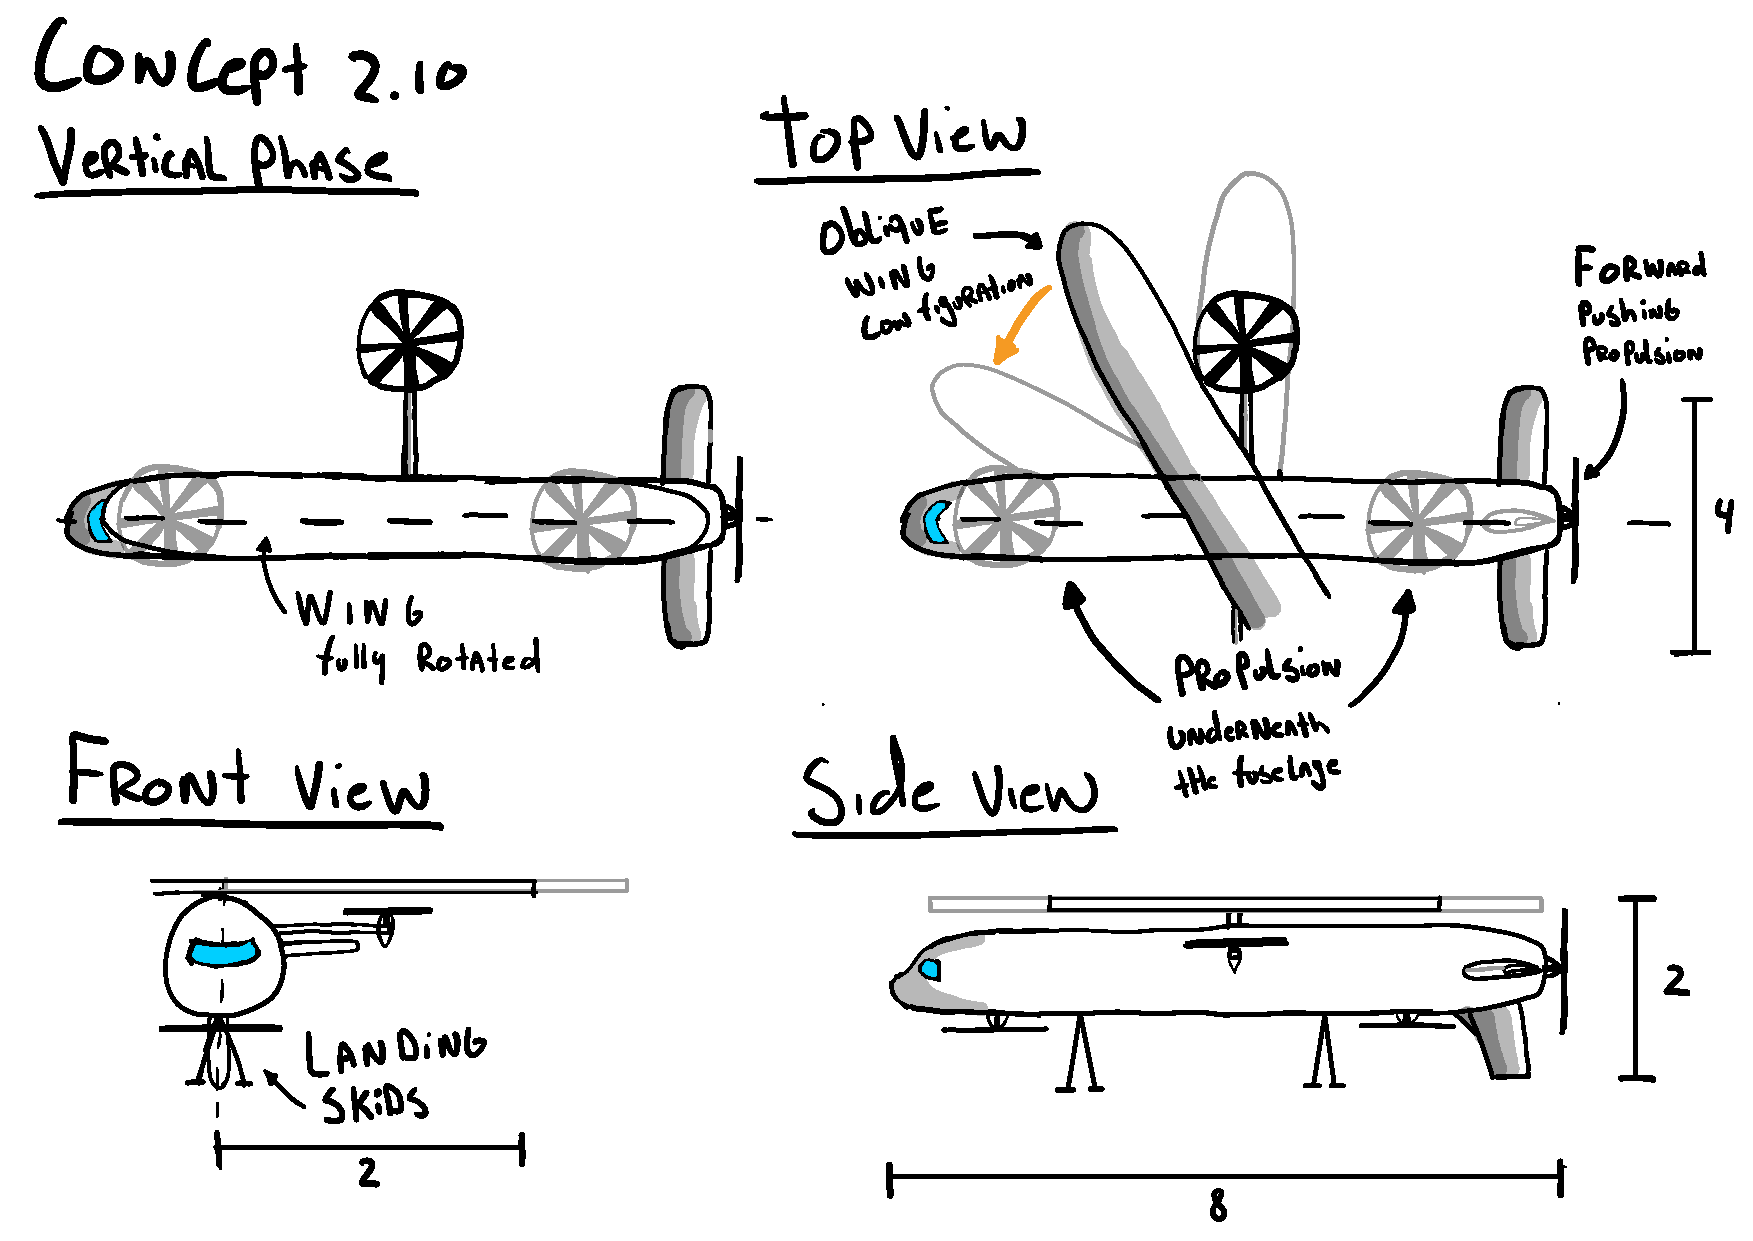
\includegraphics[width=1\linewidth]{figures/Concepts/Concept C2.10 v3.pdf}
    \caption{Concept C2.10: Variable Skew Quad Plane}
    \label{fig_oe:ConceptC2.10}
\end{subfigure}

    \caption{Concept sketches. Note: drawings are not to scale.}
    \label{fig_oe:Concept_sketches}
\end{figure}

\section*{Preliminary Sizing}
After selecting the most promising design options, it is relevant to size the different designs. This is to allow the comparison of their performance and trade off the concepts.
In order to achieve this goal, a tool has been developed that estimates several relevant characteristics. This tool comprises different parts: Class I mass estimation, Class II sizing, wing and hinge loading model, and noise estimations.

\textbf{Class I preliminary sizing} is performed first. For this, wing and power loading diagrams are constructed by setting constraints on the different mission phases as described in the mission profile. Additionally, a stall speed of 32 \unit{m/s} from CS23~\cite{easa_cs23_2020} is considered.
% An example of a wing and power loading diagram for concept C2.1 is presented:
% \begin{figure}[H]
%     \centering
%     \includegraphics[width=0.4\textwidth]{figures/PreliminarySizing/Wingloading/Concept_C1.5_(Fixed_Wing).pdf}
%     \caption{C1.5 Winged Rotorcraft}
%     \label{fig:over_C1.5WPWS}
   

%     \caption{Power and Wing Loading Diagrams for Concept C1.5}
%     \label{fig:WPWS-diagrams}
% \end{figure}
% It is clear from the diagram that the stall speed and vertical climb represent the limiting constraints on the design. This is the case for all four concepts.
\textbf{Class II sizing} follows. The sizing method used is the one described by Ugwueze et al. \cite{Ugwueze_Sizing_Method}, which relies on the Cessna II method from Roskam \cite{Roskam_Part_V}.
In order to more precisely estimate the mass of each design, the empty mass is split into three different sub-masses: energy system mass, airframe mass, and propulsion system mass.
For the airframe mass, empirical formulas are used, and the landing gear mass is determined based on the USAF method.
The propulsion system mass is also determined empirically based on the number of engines, maximum power and preliminary propeller characteristics. These sizing procedures yielded preliminary design parameters as presented in \Cref{tab:over_param}.

\textbf{Hinge loading} calculations are performed as considered a limiting aspect of the design. Three load cases are considered: cruise, hovering, and vertical take-off. Hinges positioned on the wing and in case of rotating engines are accounted for. Based on these load cases, \Cref{tab:over_load} showcases the values obtained for the maximum shear and bending loads on the mechanisms for each concept.

\textbf{A noise model} is finally implemented as the noise generated by each aircraft has to be estimated. Engine-produced noise is calculated using empirical formulae. The dependency on engine power, propeller diameter, rotational speed, and number of blades are accounted for. The results of this process are shown in \Cref{tab:over_noise}, where all configurations are represented.
In addition to this, the aerodynamic noise is considered. This is assessed qualitatively and considered to be caused mainly by the placement of aircraft surfaces with respect to the inlet and wake of the engines.

% Thus, each of the components has to be individually estimated. Regarding the energy system mass, the required power of each phase of the design, as described in the mission profile, is determined. This value shall then be multiplied by the time duration of each phase to obtain the total energy required for each phase:
% \begin{equation}
%     E_{ph} = P_{ph} \cdot t_{ph}
% \end{equation}
% These energies are then summed up to calculate the total energy, based on which the mass of the battery is determined considering a minimum state of charge ($\operatorname{SoC}_{\min}$=20\%) and a specific energy density SED = 300 Wh/kg:
% \begin{equation}
%     m_b = \frac{E_{tot}(1+\operatorname{SoC}_{\operatorname{min}})}{\operatorname{SED}\cdot\eta_{bat}}
% \end{equation}

\begin{table}[H]
\centering
\caption{Main parameters of each concept resulting from Class I and Class II sizing.}
\label{tab:over_param}
\sisetup{table-format=4.1, table-auto-round}
\begin{tabular}{lc|S|S|S|S}
\toprule
\multicolumn{2}{c|}{\textbf{Parameter}}   & \textbf{\ref{C1.5}} & \textbf{\ref{C2.1}} & \textbf{\ref{C2.6}}  & \textbf{\ref{C2.10}}   \\ \midrule
Wingspan & {[}m{]}                        & 12      & 14      & 12      & 8       \\
Wing surface & {[}m$^2${]}                  & 20.6    & 25.4    & 21.2    & 16.0    \\
Take-off power & {[}kW{]}                 & 319.6   & 582.9   & 445.1   & 455.4   \\
Total energy & {[}kWh{]}                  & 67.0    & 73.2    & 66.9    & 78.4    \\
Total mass & {[}kg{]}                     & 1210 & 1500 & 1250 & 1540 \\
Battery mass & {[}kg{]}                   & 315  & 345  & 315  & 369  \\
Airframe mass & {[}kg{]}                  & 368  & 541  & 367  & 604  \\
Propulsion mass & {[}kg{]}                & 132  & 211  & 169  & 165  \\ \bottomrule
\end{tabular}

\end{table}


\begin{table}[h]
    \centering
    \caption{Results from mechanism loading analysis}
    \label{tab:over_load}
    \begin{tabular}{l|r|r}
        \toprule
        Concept                       & Maximum Shear load {[}N{]} & Maximum Bending Load {[}Nm{]} \\ \midrule
        \ref{C1.5}: Winged Rotorcraft       & 4500                       & 1200                          \\
        \ref{C2.1}: Rotating Wing           & 7500                       & 24000                         \\
        \ref{C2.6}: Folding Wing            & 4600                       & 4600                          \\
        \ref{C2.10}:Variable Skew Quad Plane & 11300                      & 0                             \\ \bottomrule
    \end{tabular}
    
\end{table}

\begin{table}[h]
\centering
\caption{Engine noise level for each design}
\label{tab:over_noise}
\begin{tabular}{c|r|r|r|r}
\toprule
       & \ref{C1.5}  & \ref{C2.1}  & \ref{C2.6}  & \ref{C2.10} \\ \midrule
Noise level {[}dB{]} & 122.7 & 125.2 & 120.6 & 134.2 \\ \bottomrule
\end{tabular}

\end{table}

% In order to get a quantitative measure of noise generated by an engine in deribels(dB), the following equation can be used\cite{midtermnoise}:
% \begin{equation} \label{eq4}
%     \mathrm{SPL}_{1, \max }=83.4+15.3 \log _{10} P_{b r}-20 \log _{10} D+38.5 M_t-3(B-2)+10 \log _{10} N_p
% \end{equation}
% In \Cref{eq4}, the following parameters have to be inputed:
% \begin{table}[H]
% \caption{Noise model parameters}
% \centering
% \begin{tabular}{ccc}
% \hline
% Parameter & Unit & Description                     \\ \hline
% SPL       & dB   & Sound pressure at 1 meter       \\ 
% Pbr       & kW   & Engine power                    \\ 
% D         & m    & Propeller diameter              \\ 
% B         & -    & Number of blades                \\ 
% Np        & -    & Number of propellers per engine \\ 
% Mt        & -    & Rotational tip mach number      \\ \hline
% \end{tabular}
% \end{table}
% This equation can then be used to calculate the total noise of each configuration can be determined using the following method, where L represents the noise in dB:
% \begin{equation}
%     L_{t o t}=10 \log _{10}\left(\sum_{i=1}^n 10^{\left(L_{p r o p}, i / 10\right)}\right)
% \end{equation}

\section*{Trade-Off}
After the preliminary sizing of the concepts, performing the trade-off to choose the best-performing design for further development becomes possible. A careful definition of selection criteria and their respective weights is carried out. These are mainly based on the requirements defined in \cite{baselinerepo}.
%For example, based on the range requirement of 100 km, the total energy consumption can be calculated and traded-off to minimise energy requirements. Additionally, based on the reduced ground footprint requirement of 8x4x2 $m^3$, criteria CR-02 (Transition efficiency)  can be defined.
The criteria chosen are as follows: TRL (CR-01), transition efficiency (CR-02), structural complexity (CR-03), energy efficiency (CR-04), safety (CR-05), and noise emissions (CR-06). In order to improve the quality of the trade-off process, some criteria are divided into sub-criteria, each having a relative weight in the final grade of the \enquote{parent} criterion.

Each criterion is scored based on the results obtained in the preliminary sizing, based on a scale from 1 to 5. The same grading scale is used for each sub-criterion.  Once all scores are assigned, the winning concept is established via a trade-off table.
The trade-off results are presented in \Cref{tab_oe:performtoff}.

    \begin{longtable}[c]{p{2.8cm}|p{1.1cm}|p{2.1cm}|p{1.5cm}|p{1.8cm}|p{1.1cm}|p{1.5cm}|p{1.1cm}}
    \caption{Final trade-off table}
    \label{tab_oe:performtoff}\\
    \diagbox[width=3.2cm]{Concepts}{Criteria}
                             & CR-01 & \centering CR-02 & \centering CR-03 & \centering CR-04 & \centering CR-05 & \centering CR-06 & Final score\\ \hline
    \endfirsthead
    %
    \endhead
    %
    C1.5 (Winged   Rotorcraft) & \cellcolor[HTML]{83C77D}Full-sized model (4)    & \cellcolor[HTML]{E0E383}Excellent control, low CEF\footnote{conversion effectiveness factor} (3)   & \cellcolor[HTML]{E0E383}6 moving parts, low complexity, low loads (3)   & \cellcolor[HTML]{83C77D}Energy consumption  67.0 kWh (4) & \cellcolor[HTML]{63BE7B}Full redundancy (5) & \cellcolor[HTML]{E0E383}Engine noise  122.7 dB, obstruction area  9$\text{m}^2$ (3) & \cellcolor[HTML]{b2d580} \textbf{3.5}\\ \hline
    C2.1 (Rotating Wing) & \cellcolor[HTML]{E0E383}Scale model highly tested (3)  & \cellcolor[HTML]{63BE7B}Good control, excellent CEF (5)            & \cellcolor[HTML]{E0E383}2 moving parts, low complexity, high loads (3)     & \cellcolor[HTML]{E0E383}Energy consumption  73.2 kWh (3) &\cellcolor[HTML]{E0E383}Fatal hinge failure (3)&    \cellcolor[HTML]{83C77D}Engine noise  125.2 dB, obstruction area  0.5$\text{m}^2$ (4)   &  \cellcolor[HTML]{9ace7e} \textbf{3.75}         \\ \hline
    C2.6 (Folding Wing) & \cellcolor[HTML]{83C77D}Full-sized model (4)  & \cellcolor[HTML]{E0E383}High control, low CEF (3)            & \cellcolor[HTML]{FCBF7B}6 moving parts, high complexity,  medium loads (2)     & \cellcolor[HTML]{83C77D}Energy consumption  66.9 kWh (4) &\cellcolor[HTML]{63BE7B}Full redundancy (5)&    \cellcolor[HTML]{E0E383}Engine noise  120.6 dB, obstruction area  7.1$\text{m}^2$ (3)   &\cellcolor[HTML]{c9dc82} \textbf{3.35}           \\ \hline
    C2.10 (Variable Skew Quad Plane) & \cellcolor[HTML]{FCBF7B}Scale model (2)  & \cellcolor[HTML]{E0E383}High control, low CEF (3)            & \cellcolor[HTML]{83C77D}1 moving part, low complexity, medium loads (4)     & \cellcolor[HTML]{FCBF7B}Energy consumption  78.4 kWh (2) &\cellcolor[HTML]{83C77D}Fail-safe (4)&    \cellcolor[HTML]{FCBF7B}Engine noise  134.2 dB, obstruction area  6$\text{m}^2$ (2)     &\cellcolor[HTML]{eed17f} \textbf{2.8}         \\  
    \end{longtable}
As it can be seen, concept C2.1 (Rotating Wing) is the winning concept of the trade-off and is thus selected for further analysis.

\section*{Sensitivity Analysis}
In order to prove the validity of the trade-off and that the correct concept is chosen, a sensitivity analysis was performed.
First, the sensitivity of the criteria was analysed by removing one criterion and performing the trade-off with the five remaining ones. The case in which transition efficiency was removed was found to be the only scenario in which the Winged Rotorcraft would be the winner.

After the criteria are validated, it is necessary to assess the impact of each of the weights on the outcome of the trade-off.
This is performed by altering the weight of the criteria as well as taking into account that the weights still need to add up to 1.00. Additionally, the weights must constrained in a range of ±0.05 from the initial value. The Rotating Wing design proved to
be the best of all options in 98\% of the possibilities, hence clearly showing the validity of the procedures.

% Based on this, it can be seen that the rotating wing design wins the trade-off 98\% of the time which proves that the correct design has won the trade-off. 
% The grade distribution per concept is showcased in a Kernel Density plot \Cref{fig_oe:KDP} in order to present the winning concept.
% \begin{figure} [H]
%     \centering
%     
\includegraphics[width=0.5\linewidth]{figures/sensitivity.pdf}
%     \caption{Kernel density plot with final grade distributions for each concept}
%     \label{fig_oe:KDP}
% \end{figure}

\section*{Verification and Validation}
% The Verification and Validation (V\&V) process is a crucial part of the project, ensuring that the design meets all the specified requirements and that the model predictions match the real-world data.

% In the Verification process, the correctness of the implementation of the model is checked.
The verification of the preliminary sizing tool involved unit tests and equation verification.
Sanity tests ensured positive mass and non-negative energies.
Sample data was used to verify function outputs.
In the hinge load model, manual calculations were compared with code outputs for verification.
Unit consistency was checked throughout the code, especially when results seemed off.
The sources and equations were also verified.
For instance, during Class II sizing, the sizing method was found to be based on imperial units, requiring code adaptation and unit conversion.

The Validation process involves comparing the model predictions with real-world data, which is done by comparing the results of the preliminary sizing tool with literature data.
The mass breakdown diagrams of the different concepts are compared with the mass breakdown of a tilt-rotor aircraft from Kadhiresan et al.~\cite{Kadhiresan_Duffy_2019}.
The battery mass of the tilt-rotor aircraft is 25.7\% of the total mass, which is in line with the battery mass of the different concepts.
The engine mass estimation is compared to data from the literature on electric motors.
The energy consumption model is validated by comparing the energy consumption of the different concepts with Joby mission data from James Wang~\cite{weightperformanceslides}.
The cruise energy of the different concepts aligns with the energy analysis of the Joby aircraft.

For future verification and validation, the following steps are recommended:
\begin{itemize}
    \item More comparison to literature data for mass and energy breakdown.
    \item CAD model analysis, to compare the mass distribution of the concepts to the mass distribution of the CAD models.
    \item Computer simulations, to verify the energy consumption and asses the performance and stability of the concepts.
    \item The creation of a three-dimensional physical model, to do testing in a real-world environment.
    \item Unit tests for the code base, to verify the correctness of the code.
    \item Research and validate the hinge-loading based on current folding wing aircraft.
\end{itemize}

\section*{Interfaces}
% Defining the interfaces of this project is used to keep track of all connections throughout the design, insufficiently defining interface connections can lead to problems. With the help of an N2 chart, software, communication, and hardware diagrams, the interfaces of the design become clearer, enabling an easier detailed design phase. 

% In this overview, only the N2 chart is presented, since the rest of the diagrams are derived based on the interactions showcased in the chart.

All the connections throughout the design are tracked.
Software, communication, hardware diagrams, and an N2 chart are made to visualise these connections.
The N2 chart, which established the basis for the rest of the diagrams, is shown in \Cref{fig_eo:N2chart}.

\begin{figure}[ht]
    \centering
    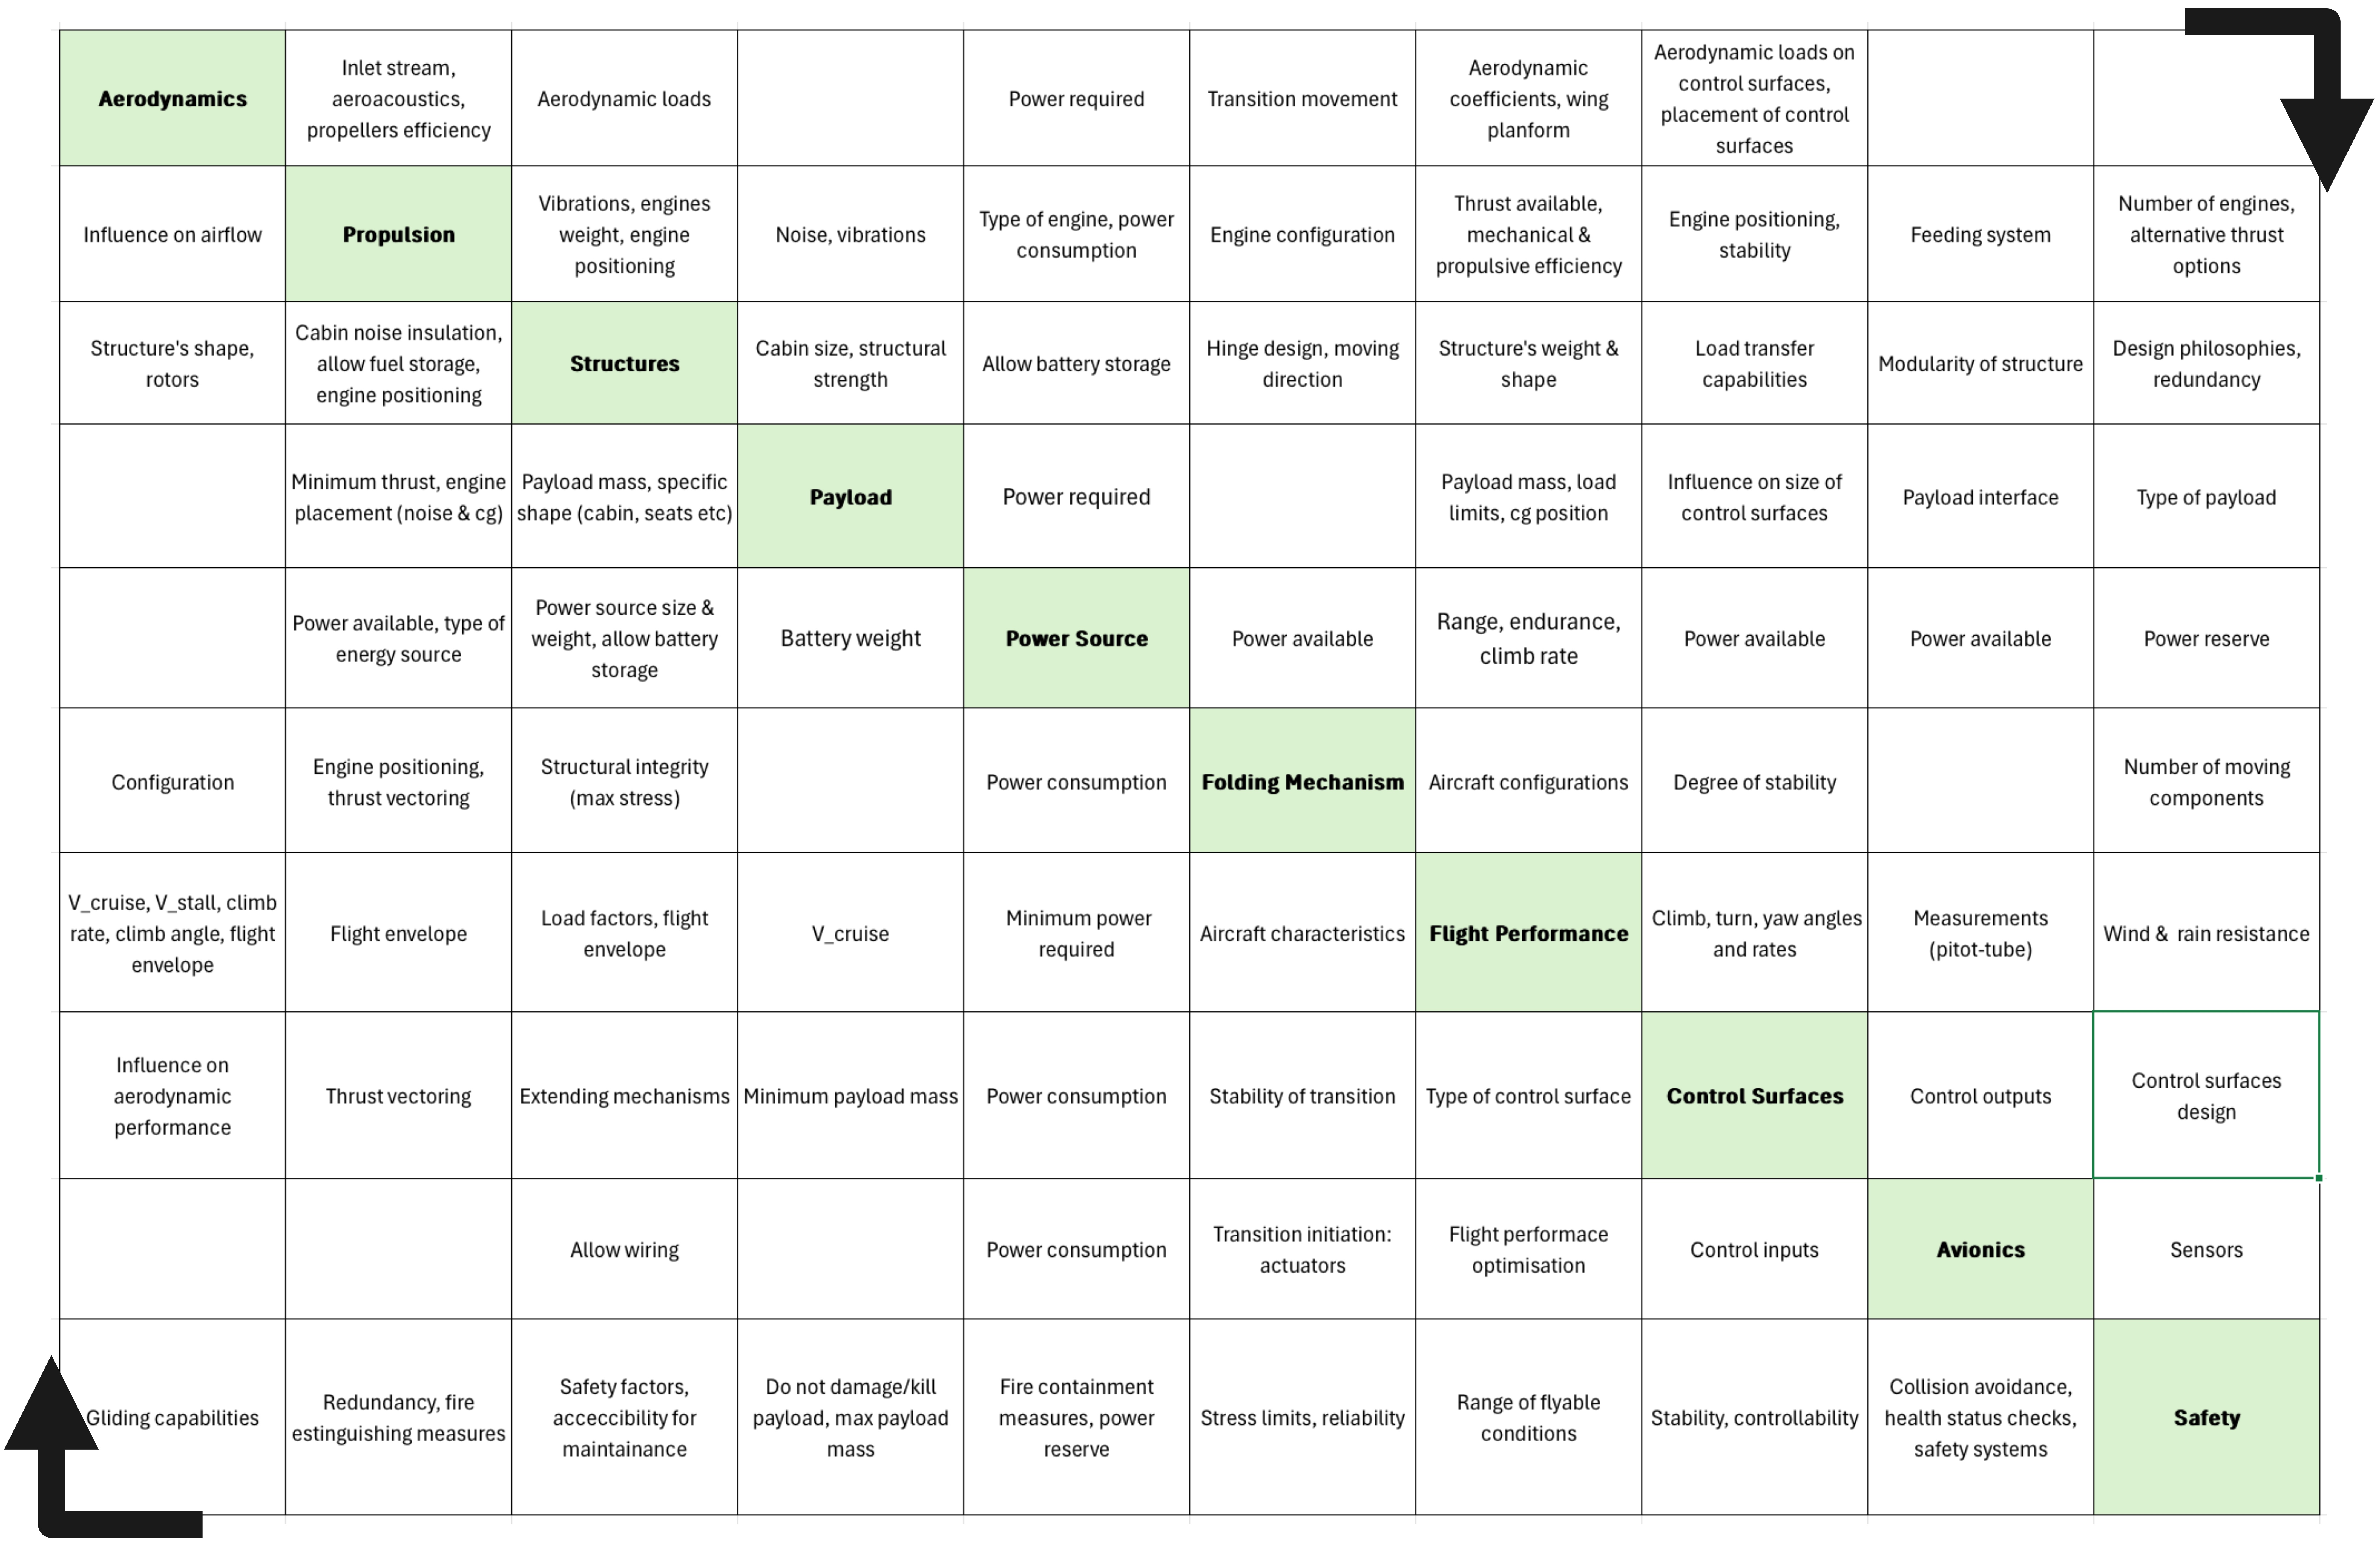
\includegraphics[width=\linewidth]{figures/N2-chart.jpg}
    \caption{N2 chart of (sub)systems}
    \label{fig_eo:N2chart}
\end{figure}

\section*{Technical Risk Assessment}
The identified risk events are distributed into five periods according to when their occurrence is expected.
These periods are the design phase, production, testing operation, and end of life. Furthermore, the risks are categorised into three types: technical, production and logistic risks. Subsequently, the impact and likelihood of the events are scored and reported on a scale of 1 to 5.
Finally, a mitigation strategy is planned, and a post-mitigation likelihood and impact are evaluated.
Some of the most critical risks are presented in \Cref{tab:critical_risks}.

\begin{table}[h]
\caption{High likelihood and impact risk events}

\label{tab:critical_risks}
\resizebox{\textwidth}{!}{%

\begin{tabular}{lccllccS[table-format=1.1]}
\hline
Risk ID   & Period      & Category   & Risk Description                                 & Impact Description                                            & \multicolumn{3}{c}{Unmitigated Risk}\\
          &             &            &                                                  &                                                               & Likelihood       & Impact & Risk \\ \hline
PR-PRD-2  & Production  & Production & Subcontractor does not meet deadlines            & Delay of construction of the vehicle, testing and operations  & 3                & 4      & 2,4  \\
PR-PRD-5  & Production  & Production & The required material is unavailable             & Delay of production                                           & 3                & 4      & 2,4  \\
PR-PRD-6  & Production  & Production & Increase in  material costs                      & Extra induced costs                                           & 4                & 3      & 2,4  \\
TR-TST-1  & Testing     & Technical  & Hinge mechanism fails under wing loading         & Crash of prototype, and repair/redesign needed                & 3                & 4      & 2,4  \\
TR-TST-2  & Testing     & Technical  & Unrealistic simulation data                      & Under-performance or crash of eVTOL                            & 3                & 4      & 2,4  \\
TR-OPR-1  & Operations  & Technical  & Maintenance costs                                & Unable to use vehicles, which increases delay and costs       & 4                & 4      & 3,2  \\
TR-OPR-5  & Operations  & Technical  & Sensors provide faulty or no data                & Faulty navigation or output by systems                        & 3                & 4      & 2,4  \\
TR-OPR-8  & Operations  & Technical  & Power drainage higher than expected in-flight    & Unable to fly full range and diversion to other landing spots & 3                & 4      & 2,4  \\
TR-OPR-10 & Operations  & Technical  & Damages infrastructure during take-off / landing & Increase in maintenance, repair costs and time                & 4                & 3      & 2,4  \\
TR-OPR-11 & Operations  & Technical  & Contact with animal                              & Possible fatal crash, involving casualties                    & 3                & 4      & 2,4  \\
TR-OPR-21 & Operations  & Technical  & Cybersecurity breach                             & Harmful intentions could result in an catastrophe             & 3                & 5      & 3,0    \\
TR-OPR-23 & Operations  & Technical  & Unforeseen flight conditions                     & Aircraft damaged and uncontrollable; emergency landing        & 3                & 5      & 3,0    \\
TR-EOL-2  & End of life & Technical  & Unable to be recycled after its life             & Cannot meet  the set  sustainability goals                    & 3                & 4      & 2,4  \\ \hline

\end{tabular}%
}

\end{table}

\section*{Production Plan}
Alongside the design of a product, its manufacturing plays a crucial role in the success of a project.
For this reason, a manufacturing plan needs to be defined.

Firstly, the advantages and disadvantages of self-production and outsourcing are identified and evaluated.
This study shows how self-producing would be less dependent on supply-chain issues, make quality control easier, and preserve the intellectual property of novel technologies.
On the other hand, outsourcing production or purchasing sub-systems would bring its own advantages. For example, it could be beneficial cost-wise, while making it easier to scale the production and not require building new facilities. After the advantages and disadvantages are known, it is possible to decide for each sub-system level whether to produce it in-house or to purchase the products from a supplier.
This is done by performing a trade-off for which several parameters are considered.

Finally, the vehicle's assembly process is assessed.
In particular, all the phases of the building process have been decided and set on a qualitative timeline that only defines the succession. A more detailed production plan, comprising of production methods and times will be produced as soon as the design reaches a more mature phase.

\section*{Sustainability Strategy}
In light of pressing environmental challenges, adopting sustainable practices in the aviation industry is crucial.
As a sustainability development strategy has already been decided upon in~\cite{baselinerepo}, here, the sustainability of the trade-off is evaluated, and more in-depth strategies are established for material selection and re-usability.
The sustainable criteria and sub-criteria are considered, multiplied by their respective weight, and summed up.
This yielded a \enquote{sustainability score} to allow comparison between the different concepts.
Concept~\ref{C2.1}, the winner of the trade-off, proves itself to be the most sustainable of the four concepts.

At this design stage, a material selection strategy is deemed essential.
It is found that material environmental impact considerations are predominant in the conceptual and preliminary phase of the design, with the establishment of related requirements.
Raw material availability, together with technical and economic assessment, are only considered in the detailed phase.
The relevance of eco-indicators is highlighted, and examples are provided.
These take into account all the sustainability dimensions.

Last but not least, the approach to lifetime and re-usability will be explained.
Modularity and standardisation are found to be potential solutions for compliance with some of the key requirements.
The importance of end-of-life disassembling strategies is also highlighted.



\section*{Conclusions}
This Rotating Wing design, which includes four engines attached to a wing that folds during take-off and landing, was selected for its excellent "conversion effectiveness" and strong performance in transition efficiency, safety, and noise footprint. Verification and validation procedures confirmed the robustness of the preliminary sizing tools and trade-off analysis, with the design proving superior in 98\% of scenarios considered. The next phase will involve refining the aerodynamic properties and developing a small-scale prototype, marking a significant step toward creating a sustainable and space-efficient eVTOL for urban environments.

Limitations were identified, including reliance on preliminary data, simplified models, and speculative Technology Readiness Level (TRL) assessments. Future work should include comprehensive structural analysis, empirical noise footprint testing, detailed transition efficiency studies, and iterative design processes. Collaboration with regulatory bodies will be crucial for meeting safety and operational standards.

